\tikzset{every picture/.style={line width=0.75pt}} %set default line width to 0.75pt        

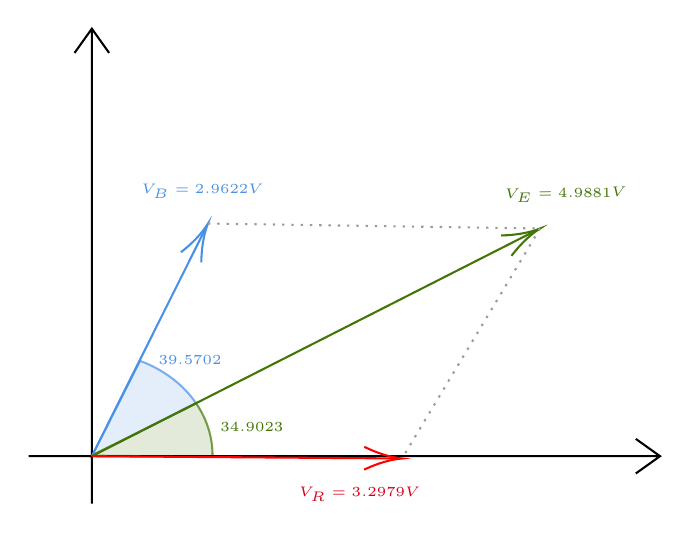
\begin{tikzpicture}[x=1.25pt,y=1.25pt,yscale=-1,xscale=1]
  %uncomment if require: \path (0,264); %set diagram left start at 0, and has height of 264

  %Shape: Pie [id:dp5796865293003781] 
  \draw  [color={rgb, 255:red, 74; green, 144; blue, 226 }  ,draw opacity=0.7 ][fill={rgb, 255:red, 74; green, 144; blue, 226 }  ,fill opacity=0.15 ] (53.94,161.7) .. controls (60.7,164.21) and (66.35,168.49) .. (70.1,173.88) -- (40,189.25) -- cycle ;
  %Shape: Pie [id:dp3559421179054527] 
  \draw  [color={rgb, 255:red, 65; green, 117; blue, 5 }  ,draw opacity=0.7 ][fill={rgb, 255:red, 65; green, 117; blue, 5 }  ,fill opacity=0.15 ] (70.16,173.99) .. controls (73.14,178.38) and (74.86,183.49) .. (74.89,188.94) .. controls (74.89,189.1) and (74.89,189.27) .. (74.88,189.43) -- (39.89,189.1) -- cycle ;
  %Shape: Axis 2D [id:dp13588485463821143] 
  \draw  (21.75,189.25) -- (204.25,189.25)(40,65.68) -- (40,202.98) (197.25,184.25) -- (204.25,189.25) -- (197.25,194.25) (35,72.68) -- (40,65.68) -- (45,72.68)  ;
  %Straight Lines [id:da02580670154590936] 
  \draw [color={rgb, 255:red, 74; green, 144; blue, 226 }  ,draw opacity=1 ]   (40,189.25) -- (72.68,123.79) ;
  \draw [shift={(73.57,122)}, rotate = 476.53] [color={rgb, 255:red, 74; green, 144; blue, 226 }  ,draw opacity=1 ][line width=0.75]    (10.93,-3.29) .. controls (6.95,-1.4) and (3.31,-0.3) .. (0,0) .. controls (3.31,0.3) and (6.95,1.4) .. (10.93,3.29)   ;
  %Straight Lines [id:da24940551444265346] 
  \draw [color={rgb, 255:red, 65; green, 117; blue, 5 }  ,draw opacity=1 ]   (40,189.25) -- (167.79,124.33) ;
  \draw [shift={(169.57,123.43)}, rotate = 513.0699999999999] [color={rgb, 255:red, 65; green, 117; blue, 5 }  ,draw opacity=1 ][line width=0.75]    (10.93,-3.29) .. controls (6.95,-1.4) and (3.31,-0.3) .. (0,0) .. controls (3.31,0.3) and (6.95,1.4) .. (10.93,3.29)   ;
  %Straight Lines [id:da8765285222569108] 
  \draw [color={rgb, 255:red, 255; green, 0; blue, 0 }  ,draw opacity=1 ]   (40,189.25) -- (127.67,189.9) ;
  \draw [shift={(129.67,189.92)}, rotate = 180.43] [color={rgb, 255:red, 255; green, 0; blue, 0 }  ,draw opacity=1 ][line width=0.75]    (10.93,-3.29) .. controls (6.95,-1.4) and (3.31,-0.3) .. (0,0) .. controls (3.31,0.3) and (6.95,1.4) .. (10.93,3.29)   ;
  %Straight Lines [id:da2698003556584623] 
  \draw [color={rgb, 255:red, 155; green, 155; blue, 155 }  ,draw opacity=1 ] [dash pattern={on 0.84pt off 2.51pt}]  (73.57,122) -- (169.57,123.43) ;
  %Straight Lines [id:da21387838894897082] 
  \draw [color={rgb, 255:red, 155; green, 155; blue, 155 }  ,draw opacity=1 ] [dash pattern={on 0.84pt off 2.51pt}]  (169.57,123.43) -- (129.67,189.92) ;

  % Text Node
  \draw (158.52,111.1) node [anchor=north west][inner sep=0.75pt]  [font=\tiny,color={rgb, 255:red, 65; green, 117; blue, 5 }  ,opacity=1 ,rotate=-359.23] [align=left] {$\displaystyle V_{E} =4.9881V$};
  % Text Node
  \draw (53.48,109.81) node [anchor=north west][inner sep=0.75pt]  [font=\tiny,color={rgb, 255:red, 74; green, 144; blue, 226 }  ,opacity=1 ] [align=left] {$\displaystyle V_{B} =2.9622V$};
  % Text Node
  \draw (99,197.33) node [anchor=north west][inner sep=0.75pt]  [font=\tiny,color={rgb, 255:red, 208; green, 2; blue, 27 }  ,opacity=1 ] [align=left] {$\displaystyle V_{R} =3.2979V$};
  % Text Node
  \draw (76.29,178.57) node [anchor=north west][inner sep=0.75pt]  [font=\tiny,color={rgb, 255:red, 65; green, 117; blue, 5 }  ,opacity=1 ] [align=left] {$\displaystyle 34.9023\degree $};
  % Text Node
  \draw (58.41,161.35) node [anchor=west] [inner sep=0.75pt]  [font=\tiny,color={rgb, 255:red, 74; green, 144; blue, 226 }  ,opacity=1 ] [align=left] {$\displaystyle 39.5702\degree $};


\end{tikzpicture}
